
%\newpage
%\thispagestyle{empty}
%\mbox{}
\chapter{Descripción del sistema}
\label{ch:chapter2}

En este capítulo, se dará a conocer el fundamento teórico sobre el que se sustenta el sistema, en donde, se detallará cada uno de los algoritmos utilizados, además de dar a conocer el modelo de simulación basado en una función gaussiana.

\section{Modelo para la simulación} \label{Simulacion_Modelo}

Antes de describir cada uno de los algoritmos pertenecientes al sistema se va a definir la función gaussiana utilizada para la simulación de la radiación de la fuente de contaminación.

\begin{equation} \label{Funcion_Gaussiana} 
	f\left(x,y\right) = p\cdot{e}^{-\left(x-c_o\right)^{T}\cdot{M}\cdot\left(x-c_{o}\right)},
\end{equation}

en donde, $x=\left(x,y\right)$, $c_o=\left(x_{o},y_{o}\right)$ sería la posición del centro de la gaussiana. Además, 

\begin{equation}
	\begin{aligned}
	M= 	
	\begin{bmatrix}
		\frac{\cos^{2}{\theta}}{2\cdot{\sigma^{2}_{x}}}+ \frac{\sin^{2}{\theta}}{2\cdot{\sigma^{2}_{y}}} & \frac{\sin{2\cdot\theta}}{4\cdot{\sigma^{2}_{x}}}+ \frac{\sin{2\cdot\theta}}{4\cdot{\sigma^{2}_{y}}}\\\\
		
		\frac{\sin{2\cdot\theta}}{4\cdot{\sigma^{2}_{x}}}+ \frac{\sin{2\cdot\theta}}{4\cdot{\sigma^{2}_{y}}} & \frac{\sin^{2}{\theta}}{2\cdot{\sigma^{2}_{x}}}+ \frac{\cos^{2}{\theta}}{2\cdot{\sigma^{2}_{y}}}\\
	\end{bmatrix}
	\end{aligned}
\end{equation}
\\

Es una matriz definida positiva y proviene de $R\cdot{S}\cdot{R}^{T}$ con $R$ siendo la matriz de rotación ordinaria en 2D para un ángulo $\theta$ definiéndose a $S$ como:

\begin{equation}
		\begin{aligned}
	S= 	
	\begin{bmatrix}
		\frac{1}{2\cdot{\sigma^{2}_{x}}} & 0\\\\
		0 & \frac{1}{2\cdot{\sigma^{2}_{y}}}\\
	\end{bmatrix}
	\end{aligned}
\end{equation}

En donde, $\sigma^{2}_{x}$ con $\sigma^{2}_{y}$ serían a desviación típica de la gaussiana con los ejes x e y respectivamente.

\begin{figure}[htb]
  \begin{center}
    \subfigure[Función definida en 3D]{
        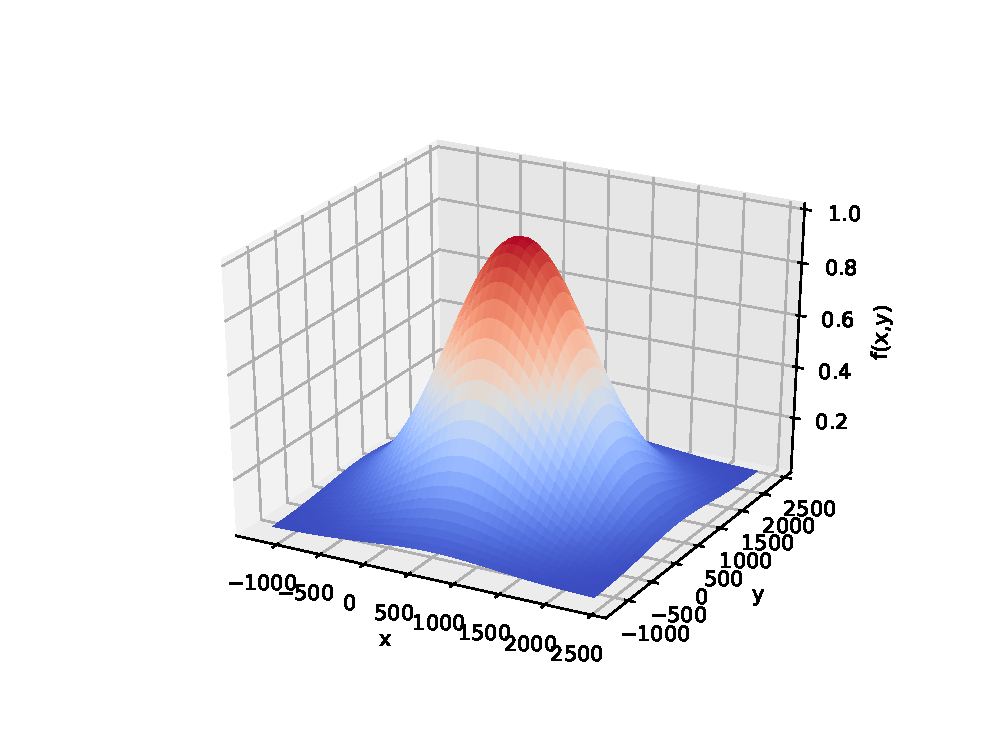
\includegraphics[width=0.45\textwidth]{figures/Gaussiana.eps}
        \label{Fgauss}}
    \subfigure[Curvas de nivel]{
        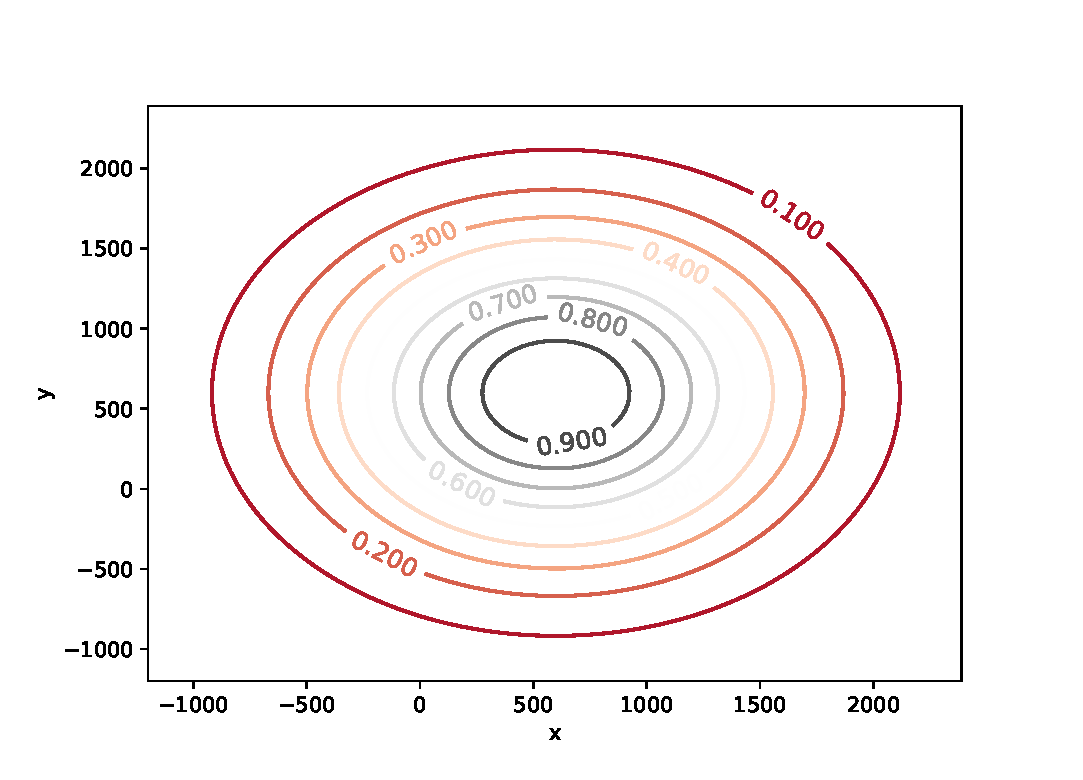
\includegraphics[width=0.45\textwidth]{figures/CurvasNivelGauss.eps}
        \label{CurvasGauss}}
    \caption{Representación de una función gaussiana}
    \label{FunGauss}
  \end{center}
\end{figure}

Se puede particularizar a un caso más sencillo para facilitar el análisis del rendimiento del sistema de la siguiente forma:

\begin{itemize}
	\item Normalizar el volumen encerrado debajo de la gaussiana para que éste tenga un valor unitario. Esto se obtiene definiendo a $p=\frac{1}{2\cdot{\pi}\sigma_{x}\sigma_{y}}$.
	\item Presentar desviaciones iguales en ambos ejes $\sigma_{x}=\sigma_{y}=\sigma$.
\end{itemize}
\newpage
Con estas dos consideraciones la expresión final sería:

\begin{equation}
	f\left(x,y\right)=\frac{1}{2\cdot{\pi}\cdot{\sigma^{2}}}e^{\frac{\left(x-x_{o}\right)^{2}+\left(y-y_{o}\right)^{2}}{2\cdot{\sigma^2}}}
\end{equation}

Esta representación es la que posteriormente se usará para las diferentes simulaciones aportadas en el capítulo \ref{ch:chapter3}. 

\section{Algoritmo de estimación de gradiente para la búsqueda de fuentes} \label{Estima}

Anteriormente se discutió que el objetivo del algoritmo es la búsqueda de fuentes, basándose en mediciones locales de múltiples robots situados de manera simétrica en un espacio de 2D. En dicho procedimiento, se consideran N robots distribuidos uniformemente a lo largo de una formación circular con un radio D y un punto central c definido en dos dimensiones, tal como se muestra en la siguiente figura \ref{Disp:Robots}.

Para la obtención del gradiente en un sistema real basta con que un único agente, a partir de la información reunida entre todos, lo estime. Sin embargo, para la simulación se utilizará la función gaussiana previamente descrita.

\begin{figure}[htb]
\centering
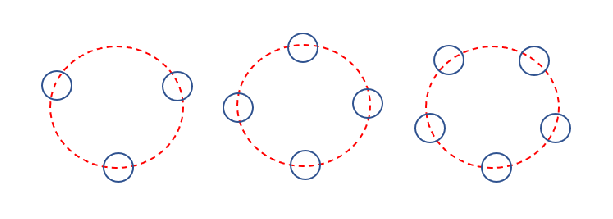
\includegraphics[width=0.95\textwidth]{figures/Disposicion_Robots.eps}
\caption{Disposición de los agentes en torno a la formación circular.} \label{Disp:Robots}
\end{figure}

Adicionalmente, cada uno de los agentes deberá tener la capacidad de medir la intensidad de la señal mediante un sensor. En términos matemáticos, la distribución de la señal es una función espacial bidimensional que representa un campo escalar con un máximo o mínimo definido justo en la posición donde dicha fuente se localiza. Por lo tanto, se va a considerar que la señal es emitida por una única fuente de modo que su punto critico en $z_*$ es el único máximo definido del campo escalar.

Por ello, es necesario definir una función $f\left(x\right)$ con $x\in\mathbb{R}^{n}$, además de ser continua y derivable para todo x. En torno a un punto $x_*$, se aplica el desarrollo en serie de Taylor para un valor de $n\geq{2}$ de la siguiente forma:

\begin{equation}\label{TaylorNormal}
	f\left(x\right)=f\left(x_{*}\right)+\mathrm{\nabla}{f}{\left(x_{*}\right)}^{T}\left(x-x_{*}\right)+\frac{1}{2!}\cdot{\left(x-x_{*}\right)}^{T}\cdot{H}\left({f}\left(x_{*}\right)\right) 		\cdot\left(x-x_{*}\right)+O\left(x_{*}^3\right)
\end{equation}

Donde:

\begin{equation*}
	\begin{aligned}
		\mathrm{\nabla}{f}=
	\begin{bmatrix}
		\frac{\partial{f}}{\partial{x}_1} \\
		\frac{\partial{f}}{\partial{x}_2}  \\
		\vdots \\
		\frac{\partial{f}}{\partial{x}_n}
	\end{bmatrix}
	\end{aligned}
	\qquad\text{y}\qquad
	\begin{aligned}
	{H}\left(f\right)=\mathrm{\nabla}^{2}{f}= 	
	\begin{bmatrix}
		\frac{\partial^{2}{f}}{\partial{x}_{1}^{2}} & \frac{\partial^{2}{f}}{\partial{x}_{1}\cdot\partial{x}_{2}} & \cdots & \frac{\partial^{2}{f}}{\partial{x}_{1}\cdot\partial{x}_{n}}\\
		\frac{\partial^{2}{f}}{\partial{x}_{2}\cdot\partial{x}_{1}} & \frac{\partial^{2}{f}}{\partial{x}_{2}^{2}} & \cdots & \frac{\partial^{2}{f}}{\partial{x}_{2}\cdot\partial{x}_{n}}\\
		\vdots & \vdots & \ddots & \vdots\\
		\frac{\partial^{2}{f}}{\partial{x}_{n}\cdot\partial{x}_{1}} & \frac{\partial^{2}{f}}{\partial{x}_{n}\cdot\partial{x}_{2}} & \cdots & \frac{\partial^{2}{f}}{\partial{x}_{n}^{2}}
	\end{bmatrix}
	\end{aligned}
\end{equation*}\\

Para evaluar el punto máximo de concentración lo que interesa es que $\mathrm{\nabla}{f}{\left(x_{*}\right)}=0$. No obstante, en el problema en cuestión no se dispone de información sobre dicho gradiente solo se tienen las medidas tomadas por los sensores en cada uno de los vehículos es por ello que se va a aprovechar para realizar una estimación del gradiente en el centro del círculo formado por los robots $\hat{\nabla}{f}\left(c\right)$.
\newpage
Particularizando para una distribución uniforme a lo largo de un circulo con radio D, un ángulo de rotación $\phi_0\left(t\right)=w_0\cdot{t}$, en el que los agentes se mueven con velocidad angular $w_0$ y el centro de la formación c. 

\begin{equation}
	r_i = c + D\cdot{R}_{\phi_i}\cdot{e}\hspace{10mm}{i = 1,...,N}
\end{equation}

Definiendo a $r_{i}$ como la posición del robot i con respecto al radio del circulo, ${\phi }_{i}=\phi_{o}+\frac{2\cdot\pi\cdot{i}}{N}$ es el ángulo de rotación, $R_{\phi }$ es la matriz de rotación definida como $\left[ \begin{array}{cc} {\cos\phi} & -{\sin\phi } \\  {\sin\phi } & {\cos\phi } \end{array} \right]$ y  $e\ =\ {\left[1,0\right]}^T$.

\begin{figure}[htb]
\centering
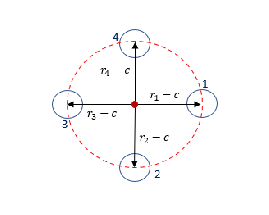
\includegraphics[width=0.5\textwidth]{figures/p3.eps}
\caption{Estrategia colaborativa para el cálculo del gradiente en el centro de la circunferencia formada por los agentes.} \label{Estrategia_Colaborativa}
\end{figure}


A partir de la ecuación \ref{TaylorNormal} pero haciendo la expansión de Taylor hasta el termino primer orden sobre cada una de las medidas $f\left(r_i\right)$ en torno al punto c y redefiniendo a $D$ como $D=||r_i-c||$, se obtiene:

\begin{equation} \label{PuntoPartidaGradiente}
	f\left(r_i\right)-f\left(c\right)=\nabla{f\left(c\right)}^T\left(r_i-c\right)+\varphi_i\left(D,c\right)\hspace{12mm}\forall{i},\cdots,N,
\end{equation}

en donde, $\varphi_i\left(D,c\right)$ denota el remanente de la expansión de Taylor. 

Para obtener una estima del gradiente se utilizan las medidas tomadas por los sensores de cada uno los vehículos $f\left(r_i\right)$ y la posición de cada uno de ellos por medio de:

\begin{equation}\label{Fun_Esti}
	\frac{2}{N\cdot{D}^2}\cdot\sum_{i=1}^{N}f(r_{i})\cdot(r_{i}-c)=\underbrace{\nabla{f}\left(c\right) + \varphi\left(D,c\right)}_{:=\hat{\nabla}{f}\left(c\right)}
\end{equation}

La obtención de dicha expresión, así como la prueba de su validez pueden encontrar en \cite{Estimacion_Gradiente} y \cite{Adicional_Estimacion_1}. En donde, $\varphi\left(D,c\right)$ es el error de la aproximación. 

Para evaluar la fiabilidad de la estima se va a comparar con el valor exacto del gradiente obtenido sobre una función gaussiana y como influye en la bondad de dicho cálculo el número de agentes empleados y el radio del círculo de la formación. Por ello, se establece una posición arbitraria para el centro de la formación  se encuentre relativamente lejos de la fuente. Así pues, se evalúa la variación del número de agentes con un radio unitario y del radio con el mínimo de número de agentes posibles.

Finalmente, se hace uso de la función \ref{Funcion_Gaussiana} cuyos valores serían $c_{o}=[600,600]$, el ángulo $\theta$ nulo, una desviación uniforme en ambos ejes $\sigma_{x}=\sigma_{y}=\frac{1}{1000}$ para que la matriz quede definida como $S = \bigl[\begin{smallmatrix}\frac{1000}{\sqrt{2}} & 0\\ 0 & \frac{1000}{\sqrt{2}}\end{smallmatrix}\bigr]$  y cuyo volumen es $p = 1$. 

\begin{figure}[H]
  \begin{center}
    \subfigure[N = 2]{
        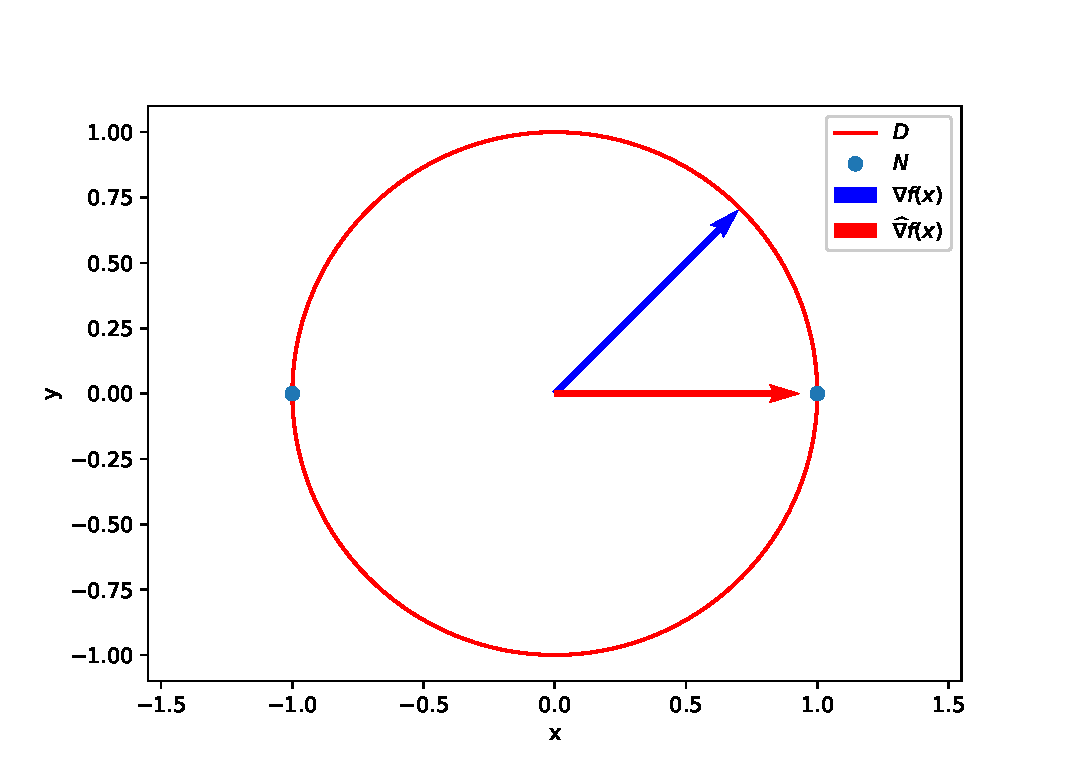
\includegraphics[width=0.38\textwidth]{figures/N2_RFIJO.eps}
        \label{N = 2}}
    \subfigure[N = 3]{
        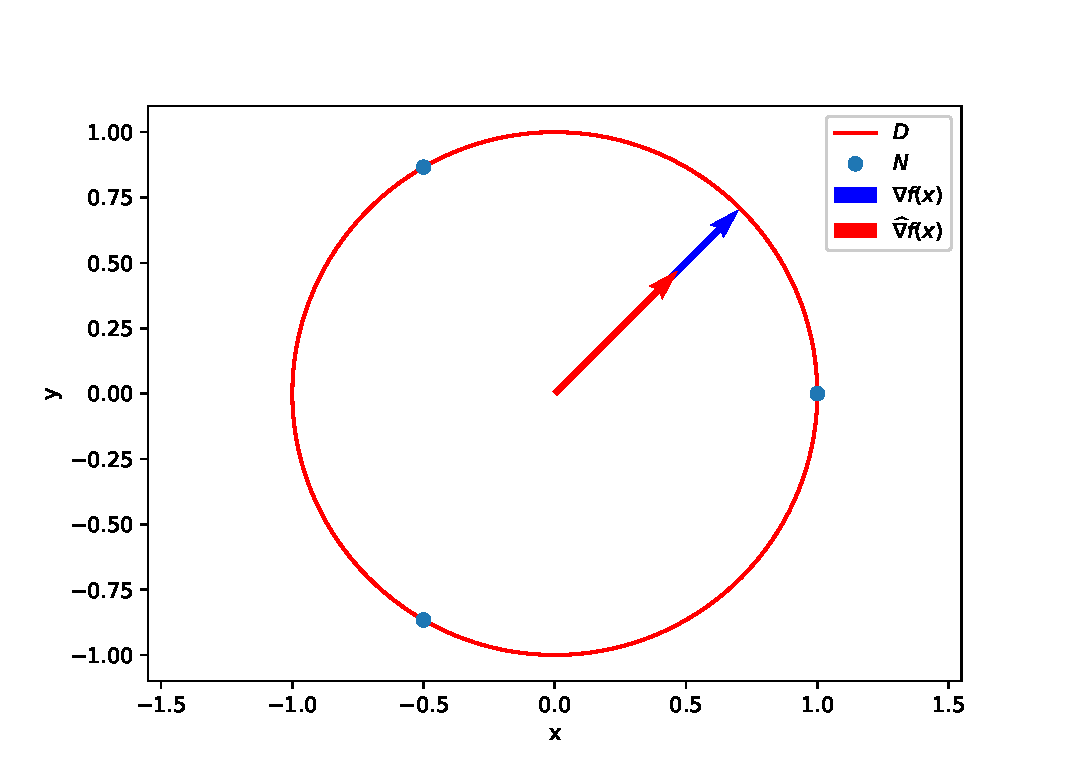
\includegraphics[width=0.38\textwidth]{figures/N3_RFIJO.eps}
        \label{N = 3}}
    \caption{Estimación del gradiente en función del número de agentes con D = 1. La figura de la izquierda es un caso no valido y se aporta para demostrar un mal uso del algoritmo.}
    \label{NAGENTSEST}
  \end{center}
\end{figure}

Se observa en la figura \ref{N = 3} que aplicar tan solo el algoritmo de estima da un error prácticamente inapreciable. Por otra parte, el algoritmo solo funciona si cooperan tres o más vehículos, tal como se anticipaba en \cite{Estimacion_Gradiente}. De manera análoga, se procede a evaluar el efecto del radio:

\begin{figure}[H]
  \begin{center}
    \subfigure[D = 100]{
        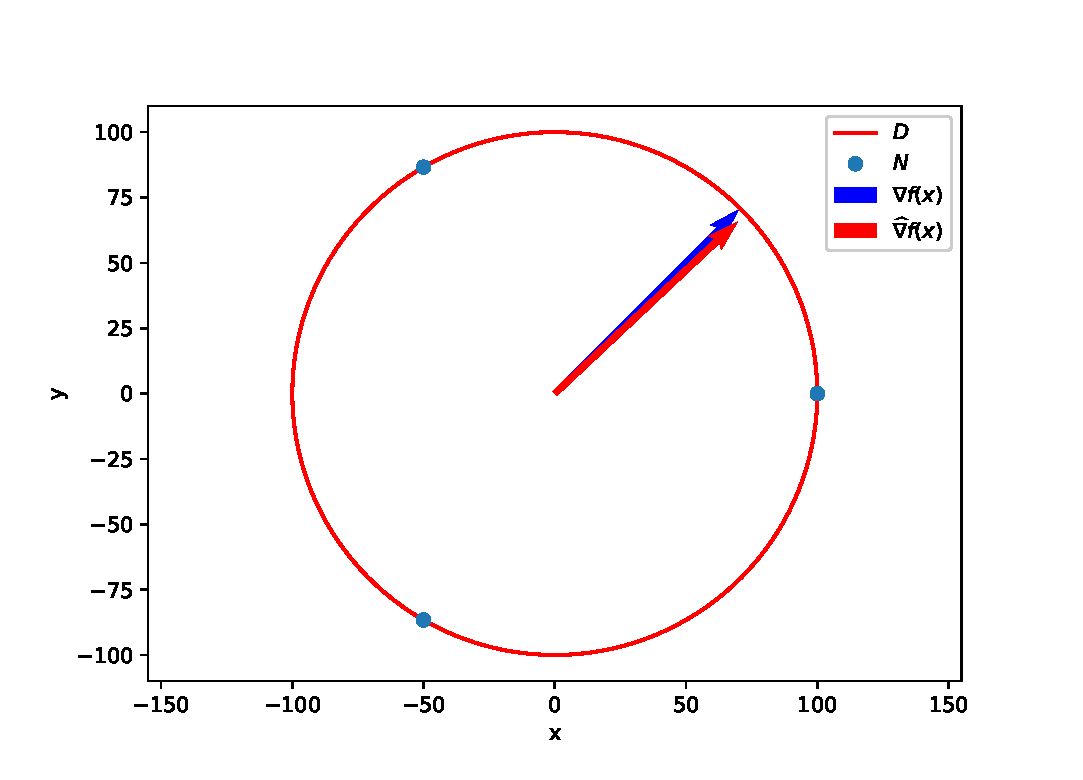
\includegraphics[width=0.40\textwidth]{figures/R100_NFIJO.eps}
        \label{D = 100}}
    \subfigure[D = 10]{
        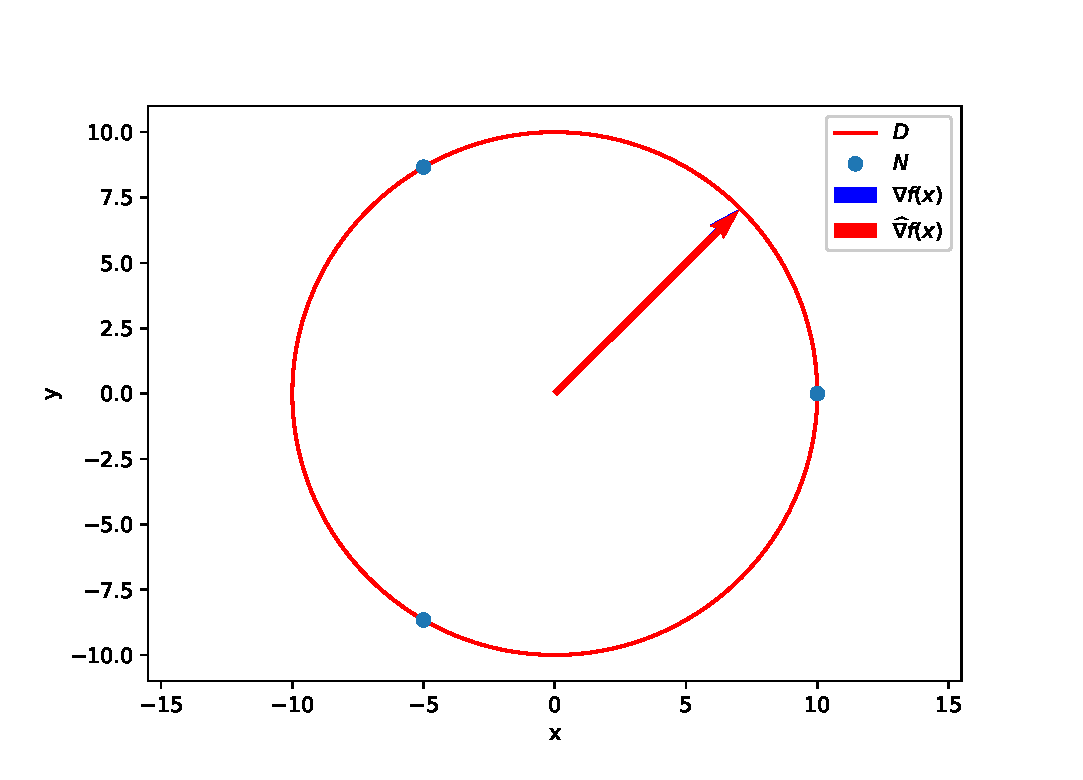
\includegraphics[width=0.40\textwidth]{figures/R10_NFIJO.eps}
        \label{D = 10}}
    \caption{Estimación del gradiente en función del radio del círculo con N = 3}
    \label{VARD}
  \end{center}
\end{figure}

En el caso de figura \ref{VARD} la relación es inversa al número de agentes, es decir, cuanto menor es el radio menor será el error. No obstante, se deben considerar las dimensiones de los vehículos dado que si el radio es excesivamente pequeño pueden generarse colisiones entre ellos.

Se destaca que en ambos casos el gradiente apunta en la dirección del centro de la gaussiana, es decir, presenta una orientación en razón de un ángulo de $\frac{\pi}{4}$ con respecto al centro de la formación ubicada en el origen.

Este método será adoptado por los vehículos de superficie marítima que giran en torno a una distancia $D$ prescrita e irán tomando medidas que se utilizan para obtener el gradiente de concentración. Para ello, es necesario definir un algoritmo que les otorgue la capacidad de coordinarse, el cual se explica a continuación.

\section{Algoritmo de control de formación circular}

El control de la formaciones tiene como objetivo conseguir que un sistema formado por múltiples vehículos naveguen manteniendo una forma geométrica deseada. Una forma particular de hacerlo es mediante algoritmos de cooperación entre los agentes.

El modelo dinámico que se utilizará considera vehículos tipo monociclo con velocidad constante, es decir, solo se actúa sobre la dirección del vehículo a través de giros coordinados actuando sobre el ángulo de orientación. Las ecuaciones del monociclo con el que se simulan los vehículos son las siguientes: 

\begin{equation} \label{Dinamica}
	 \left \{
    \begin{aligned}
\dot{p}_{i}&=u_{r}\cdot{m\left(\psi_{i}\right)}\\
\dot{\psi_{i}}&=u_{\psi_{i}},\\
    \end{aligned}
  \right.
\end{equation}

en donde, $u_{r}$ es la velocidad que ha de ser constante, además de tener el mismo valor para cada uno de los vehículos, $m=\left[\cos\left(\psi_{i}\right)\hspace{2mm}\sin\left(\psi_{i}\right)\right]^{T}$ con $\psi_{i}$ siendo el angulo de orientación y $u_{\psi_{i}}$ es la entrada de control que otorga la capacidad a cada uno de los vehículos $i$ de converger a una circunferencia deseada. Posteriormente, se explicará más detalladamente su efecto sobre cada vehículo.

Los vehículos modificarán su velocidad angular en función de girar en torno a un punto central y manipular la circunferencia que describen. De este modo, se puede hacer que aumenten o disminuyan la distancia angular entre ellos.

Definiéndose como objetivo el describir un \textbf{algoritmo distribuido para controlar formaciones circulares} aplicados a los USVs comentados en \ref{Motiv}. Es importante destacar que el algoritmo va a tener dos tareas:
\newpage
\begin{itemize}
	\item Inicialmente cada uno de los vehículos estarán en posiciones arbitrarias y deberán converger hacia la circunferencia de radio $D$ en el que vas a hacer la medida de concentración.
	\item Posteriormente, deberán mantener la misma distancia angular entre sus vecinos distribuyéndose uniformemente en torno a dicha circunferencia. Esto será posible al minimizar el error existente entre sus ángulos como más adelante se comentará.
\end{itemize}

Para la primera de las tareas se basa en la idea de un único vehículo arranque desde cualquier posición y sea capaz de converger a una circunferencia deseada.

Se debe definir una trayectoria circular de radio $D\in\mathbb{R}^+$ puede ser descrita mediante la siguiente ecuación:
\begin{equation}	
	C_D\triangleq\left\lbrace{p:\varphi{\left(p\right)}=0}\right\rbrace{,}
\end{equation}

en donde, $\varphi\left(p\right)=p_{x}^{2}+p_{y}^{2}-D^{2}$ y $p=\left[p_x\hspace{2mm}p_y\right]^T$ representa la posición cartesiana con respecto a un marco de coordenadas cuyo origen esta en el centro de $C_D$. Si $\nabla{\varphi\left(p\right)}\neq{0}\Longleftrightarrow{p}\neq{0}$ todo el conjunto de niveles $\varphi_c\left(p\right)$ se pueden parametrizar. Se puede obtener un ángulo $\theta$ asociado a la posición del vehículo mediante:

\begin{equation}
	\theta\left(p\right)=atan2\left(p_{y},p_{x}\right)\in\left(-\pi,\pi\right]
\end{equation} 

El vehículo a su vez posee dos vectores necesarios para hacerlo converger a la circunferencia deseada. El primero de ellos se atribuye a un vector normal a la circunferencia dada por $\varphi\left(p\right)$ definiéndose como $n\left(p\right)\triangleq\nabla\varphi\left(p\right)$, el otro es un vector tangente al punto $p$ y descrito por $\tau\left(p\right)=E\cdot{n\left(p\right)}$ con $E = \bigl[\begin{smallmatrix}0 & 1\\ -1 & 0\end{smallmatrix}\bigr]$ una matriz de rotación de $-\frac{\pi}{2}$. Ambos vectores son apreciables en la figura \ref{Primera_Acción_Control}. En esta se observa la elección de uno de los vectores tangentes, se debe a que la matriz $E$ otorga un sentido de giro horario y es por ello que solo se indica uno de las dos posibilidades.

\newpage
\begin{figure}[htb]
\centering
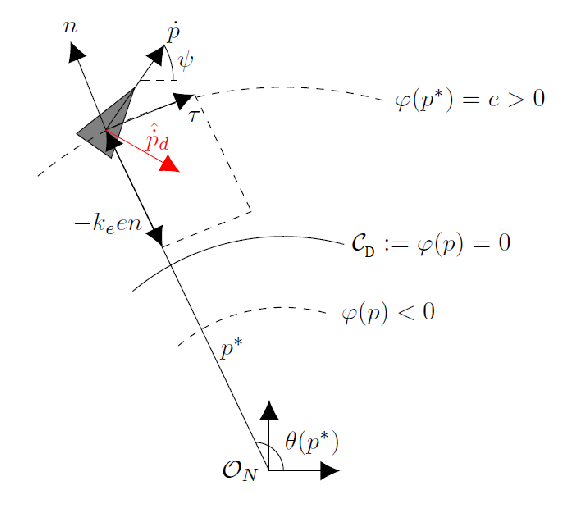
\includegraphics[width=0.60\textwidth]{figures/Coord_1.eps}
\caption{Un único vehículo con la capacidad de converger a una circunferencia destino. Figura tomada de: \cite{Control_Formacion}} \label{Primera_Acción_Control}
\end{figure}

En la figura \ref{Primera_Acción_Control} se aprecia un vector $\hat{\dot{p_d}}$. Este es un vector unitario que indica la velocidad deseada por el vehículo. Dicha velocidad modifica la orientación del vehículo para que sea capaz de ser tangencial a la trayectoria en todo punto. El vector $\hat{\dot{p_d}}$ se describe como la suma de:

\begin{equation} \label{Control_for}
	\hat{\dot{p_{d}}}\left(p\right)\triangleq\tau\left(p\right)-k_{e}\cdot{e\left(p\right)}\cdot{n\left(p\right)},
\end{equation}

en donde, $k_{e}\in\mathbb{R}^{+}$ es una ganancia que define cuan agresivo es el campo vectorial para converger a $C_D$ y $e\left(p\right)\triangleq\varphi\left(p\right)$ es el error en la distancia entre la circunferencia actual del vehículo $\varphi\left(p^*\right)$ y la circunferencia objetivo. Se derivan tres casos de la expresión \ref{Control_for}:

\begin{itemize}
	\item Si $e\left(p\right)>0$ el vehículo se encuentra en una circunferencia con mayor radio que la objetivo. Caso de la circunferencia externa en la figura \ref{Primera_Acción_Control}.\newpage
	\item Si $e\left(p\right)<0$ el vehículo se encuentra en una circunferencia con menor radio que la objetivo. Caso de la circunferencia interna en la figura \ref{Primera_Acción_Control}.
	\item Si $e\left(p\right)=0$ la orientación de la velocidad del vehículo es tangente a la trayectoria. En otras palabras, se encuentra en la circunferencia destino $\varphi\left(p\right)=0$. Caso de la circunferencia central en la figura \ref{Primera_Acción_Control}.
\end{itemize}

Para conseguir que el vehículo adquiera una orientación deseada, además de los conceptos discutidos hasta ahora, será necesario introducir una entrada de control $u_{\psi}$ vista en la ecuación \ref{Dinamica}. Esta se define como:

\begin{equation} \label{Action_Control}
	\dot{\psi}={u_{\psi}}\left(\dot{p},\dot{p_{d}}\right)=\dot{\psi_{d}}+k_{d}\cdot{\hat{\dot{p}}^{T}}\cdot{E}\cdot{\hat{\dot{p_{d}}}},
\end{equation}

en donde, $k_{d}\in\mathbb{R}^{+}$ es una constante que altera la velocidad de convergencia con la que cada vehículo viaja en torno a $C_D$. Esta entrada de control se compone de dos partes que se explican a continuación.

\begin{equation}\label{Orientacion_deseada}
\dot{\psi_{d}}=-\left(E\cdot\hat{\dot{p_d}}\cdot{\hat{\dot{p_{d}}}^{T}}\cdot{E}\left(\left(E-k_{e}\cdot{e}\right)\cdot{H\left(\varphi\right)}\cdot{\dot{p}}-k_{e}\cdot{n^T}\cdot{\dot{p}}\cdot{n}\right)\right)^{T}\cdot{E}\cdot{\frac{\dot{p_d}}{\|\dot{p_{d}}\|^{2}}}
\end{equation}

Esta expresión surge de la necesidad de relacionar la dirección deseada por el vehículo $\hat{\dot{p_{d}}}$ con su ángulo de orientación. Los detalles de la obtención de dicha expresión se pueden consultar en \cite{Base_Coorporativa}.

Por otro lado, el termino $k_{d}\cdot{\hat{\dot{p}}^{T}}\cdot{E}\cdot{\hat{\dot{p_{d}}}}$ es el producto escalar de la dirección actual del vehículo con un vector perpendicular a éste. El vector perpendicular sale de realizar el producto entre la matriz de rotación $E$ con el vector unitario de la velocidad deseada $\hat{\dot{p_{d}}}$.
\newpage
Retomando la figura \ref{Primera_Acción_Control}, el resultado de aplicar la entrada de control es buscar que el ángulo formado entre $\dot{p}$ y $\hat{\dot{p_d}}$ se haga 0, es decir, que sean paralelos y apunten tanto la dirección actual del vehículo como la deseada en la misma dirección. Esto se consigue en el momento que el vector perpendicular ${E}\cdot{\hat{\dot{p_{d}}}}$ tenga un ángulo de $\frac{\pi}{2}$ con respecto a la dirección actual del vehículo $\hat{\dot{p}}$.

Este control se aplica a cada uno de los vehículos que posteriormente componen la formación circular,  para el siguiente paso es necesario definir el grafo descrito entre dichos vehículos.

Inicialmente, se considera una formación con $N\geq{2}$ vehículos cuyas posiciones $p$ se definen por $p_i\in\mathbb{R}^2$ con $i\in\left\lbrace{1,\cdots,N}\right\rbrace$, en donde los vehículos son capaces de detectar las posiciones relativas con respecto a sus vecinos. Evaluando la relación existente entre los vecinos ésta puede describirse mediante un grafo $\mathbb{G}=\left(\mathcal{V},\mathcal{E}\right)$ siendo $\mathcal{V}=\left\lbrace{1,\cdots,N}\right\rbrace$ los distintos nodos pertenecientes al grafo, en donde cada uno de ellos representa un vehículo y $\mathcal{E}\subseteq\mathcal{V}\times\mathcal{V}$ sus aristas. El conjunto de los vecinos del vehículo $i$ esta definido por $\mathcal{N}_i\triangleq\left\lbrace{j\in\mathcal{V}:\left(i,j\right)\in\mathcal{E}}\right\rbrace$. Dos vértices son adyacentes si $\left(i,j\right)\in\mathcal{E}$. Un camino desde el nodo $i$ hasta el nodo $j$ es una secuencia que comienza en $i$ y termina en $j$, de manera que dos vértices consecutivos son adyacentes, y si $i=j$ el camino se le conoce como ciclo. \cite{Control_Formacion}

Asumiendo que el grafo $\mathbb{G}$ esta conectado, es decir, existe un camino que conecta a cada par de nodos $i$ y $j$. Se definen los elementos de la matriz de incidencia $B\in\mathbb{R}^{|\mathcal{V}|\times|\mathcal{E}|}$, donde $|\chi|$ representa la cardinalidad del conjunto $\chi$, para $\mathbb{G}$ dado por:

\begin{equation} \label{Incidence}
  b_{ik}\triangleq\left \{
    \begin{aligned}
+1\hspace{5mm}si\hspace{5mm}i&=\mathcal{E}^{cola}_{k}\\
-1\hspace{5mm}si\hspace{5mm}i&=\mathcal{E}^{cabeza}_{k},\\
0\hspace{10mm}c.c\\
    \end{aligned}
  \right .
\end{equation}

en donde $\mathcal{E}^{cola}_{k}$ y $\mathcal{E}^{cabeza}_{k}$ representa los nodos cola y cabeza de la arista $\mathcal{E}_{k}$, es decir, $\mathcal{E}_{k}=\left(\mathcal{E}^{cola}_{k},\mathcal{E}^{cabeza}_{k}\right)$. 

A continuación, la figura \ref{Grafo_Demostracion} ilustrará un grafo formado por cuatro vehículos cuya matriz de incidencia se define como:

\begin{equation} \label{Incidence_Matrix}
	\begin{aligned}
	{B}= 	
	\begin{bmatrix}
		 1 &  0  &  0\\
		-1 &  1  &  0\\
		 0 & -1  &  1\\
		 0 &  0 &  -1\\
	\end{bmatrix}
	\end{aligned}
\end{equation}

Se destaca que van a estar conectados todos los nodos adyacentes salvo el primero con el último.

\begin{figure}[H]
\centering
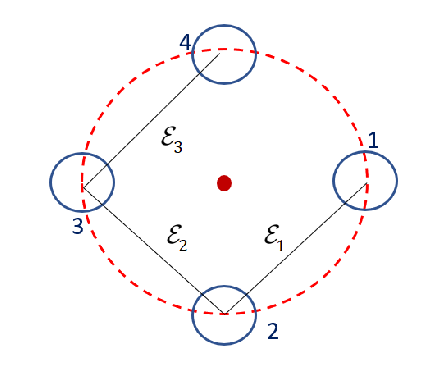
\includegraphics[width=0.45\textwidth]{figures/Grafo.eps}
\caption{Grafo descrito por 4 vehículos. Definido por los nodos $\mathcal{V}=\left\lbrace{1,2,3,4}\right\rbrace$ y las aristas $\mathcal{E}_1$, $\mathcal{E}_2$ y $\mathcal{E}_3$} \label{Grafo_Demostracion}
\end{figure}

Una vez descrita la capacidad de convergencia asociada a cada vehículo y el grafo formado por estos. Se introduce la capacidad de disponerse uniformemente en torno a la formación circular. Para ello se dispone de la velocidad angular definida para cada uno de los vehículos:

\begin{equation}
	\dot{\theta}_{i}=\omega_{i}=\frac{u_{r}}{r},
\end{equation}

en donde, $u_{r}$ es la velocidad lineal que ha de ser constante como se describió al principio de la sección y $\dot{\theta}_{i}$ es la velocidad angular asociada a cada vehículo.
\newpage

\begin{figure}[H]
\centering
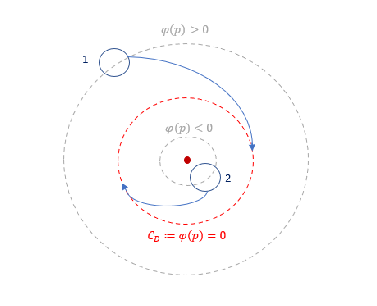
\includegraphics[width=0.60\textwidth]{figures/Pruea_Coordinacion.eps}
\caption{Disposición de dos vehículos orbitando en dos circunferencias diferentes y alterando su velocidad angular para converger circunferencia objetivo.} \label{Ejemplo_Coordinacion}
\end{figure}

La idea es controlar el ángulo entre vehículos $z = B^{T}\cdot\theta$ modificando la trayectoria descrita. Se define:

\begin{equation}\label{Control}
	C_i\left(D,c_{i}\right)\triangleq\left\lbrace{p:\varphi\left(p\right)=c_{i}}\right\rbrace,
\end{equation}

en donde, $c_i \in \mathbb{R}$ es la señal de control de formación y el subindice $i\in\mathcal{V}$ denota cada uno de los vehículos. A partir de dicha ecuación surgen dos situaciones:

\begin{itemize}
	\item Si $c_i$ es positivo, el radio D tenderá a aumentar y con ello se reduce la velocidad angular $\dot{\theta}_i$. Situación del agente 1 en la figura \ref{Ejemplo_Coordinacion}
	\item Si $c_i$ es negativo, el radio D tenderá a disminuir y con ello se aumenta la velocidad angular $\dot{\theta}_i$. Situación del agente 2 en la figura \ref{Ejemplo_Coordinacion}
\end{itemize}
\newpage
Se define a $c_i\triangleq{^{i}u}_{D}^{2}+2D\cdot{^i}u_{D},$ donde $^{i}u_{D}\in\mathbb{R}$ es una acción de control que posee un significado físico más directo al imponer el radio de la circunferencia de la siguiente forma:

\begin{equation} \label{Circulo_Neg}
	x^2+y^2-D^2={^{i}}u_{D}^{2}+2D{^{i}}u_{D} \Leftrightarrow x^2+y^2-(D+{^{i}}u_{D})^2
\end{equation}

La acción de control adquiere el siguiente significado ${^{i}}{u}_{D}=k_{r}\sum_{i=1}^N{B_i}\cdot{e}$, definiendo a $B_i$ como cada una de las filas de la matriz de incidencia \ref{Incidence}, $k_r\in\mathbb{R}^{+}$ es una constante proporcional al error que se quiere corregir y $e$ se corresponde con el error en la distancia angular entre vehículos descrito como: 

\begin{equation} \label{Error_Coordinacion}
	e_{\theta_{k}}\left(t\right)=z_{k}\left(t\right)-z_{k}^{*},
\end{equation}

en donde, $e_{\theta_{k}}\in\left(-\pi,\pi\right]$ con $k\in\left\lbrace{1,\cdots,|\mathcal{E}|}\right\rbrace$, $z_{k}^{*}$ es la distancia angular deseada y $z_{k}\left(t\right)$, previamente descrito, es la distancia angular deseada.

Un aspecto a considerar es que se impone sobre $k_{r}$ la condición de $r-\pi\cdot{k_{r}}max\left(\left\lbrace\mathcal{N}_{i}\right\rbrace\right)>0$. Esta impide la posibilidad de tener radios negativos en \ref{Circulo_Neg}.

El propósito de este control es permitir a los vehículos orbitar en torno a diferentes circunferencias en función del error existente en la distancia angular entre vehículos adyacentes. Este error va a actuar sobre el ángulo de orientación del vehículo descrito en la ecuación \ref{Action_Control} por medio de la expresión \ref{Orientacion_deseada}. Seguidamente, se dan dos posibles situaciones que pueden darse en base a todo lo definido hasta este punto:

\begin{itemize}
	\item Si el error entre dos vehículos es positivo, el vehículo se encuentra orbitando en una circunferencia con mayor radio que la objetivo. Esto se traduce en una reducción en la velocidad angular $\omega_{i}$ correspondiente al vehículo $i$.\newpage
	\item Si el error entre dos vehículos es negativo, el vehículo se encuentra orbitando en una circunferencia con menor radio que la objetivo. Esto se traduce en un aumento en la velocidad angular $\omega_{i}$ correspondiente al vehículo $i$.
\end{itemize}

El objetivo final del algoritmo es que cuando $t\rightarrow\infty$ se tenga que $e_{\theta}\rightarrow{0}$ y $p_{i}\left(t\right)\rightarrow{C_D}$, en otras palabras, que pasado un tiempo el error sea el mínimo posible permitiendo que cada uno de los vehículos este dispuesto uniformemente a lo largo de la circunferencia. Esto se traduce en que la diferencia entre el ángulo entre vehículos real y el deseado se minimice. 

\section{Algoritmo de ascenso de gradiente}

Hasta el momento únicamente se ha comentado sobre la cooperación de los agentes para la disposición de una figura geométrica y simétrica requerida o un algoritmo para la estima del gradiente en un punto. No obstante, se ha dejado de lado el avance de los agentes, es decir, ha de existir un algoritmo que desplace a todo el enjambre hacia la ubicación de la fuente haciendo uso del gradiente estimado.

Para ello, se utiliza el algoritmo de ascenso de gradiente su objetivo principal es desplazar el centro de la formación circular dado que sobre éste se encuentra definido el gradiente, la ecuación que lo describe presenta la siguiente forma \cite{Adicional_Estimacion_1}:

\begin{equation}\label{GA}
	c_{k+1}=c_k+\epsilon\cdot\nabla{f}\left(c_k\right)\hspace{10mm}c_k=[x,y]\hspace{2mm}\forall_{x,y}\in\mathbb{R},
\end{equation}

en donde, $c_k$ corresponde con el centro de la formación circular y $\epsilon\in\mathbb{R}^{+}$ es una constante que modifica la magnitud de avance gradiente. Al tratarse de un problema definido como un punto máximo de una función, el avance ha de ser estrictamente positivo, es decir, los valores de la función han de ser cada vez mayores para desplazarte hacia dicho punto.

\section{Operación conjunta de los tres algoritmos.}

\begin{figure}[H]
\centering
\includegraphics[width=0.78\textwidth]{figures/Flujo2.eps}
\caption{Diagrama de flujo que describe la dinámica del sistema.} \label{fig:Flujo}
\end{figure}

En la figura \ref{fig:Flujo} se pueden apreciar diferentes colores para diferenciar cada uno de los pasos a seguir antes de que los USVs lleguen a la zona con máximas sustancias contaminantes, desglosándolos estos serían:
\newpage
\begin{enumerate}
	\item Se disponen los N agentes en el plano, es decir, se conoce la posición de cada uno de los USV en la superficie marítima.
	\item Se ejecuta el algoritmo de control de formación circular para hacer que convergan cada uno de los vehículos a la circunferencia deseada y a su vez se dispongan de manera uniforme. Un aspecto a destacar es que se tiene que poner un umbral para decidir cuando avanzar. Dicho umbral esta estrictamente relacionado con el error de la formación descrito en la ecuación \ref{Error_Coordinacion}
	Si este valor es lo suficientemente pequeño el enjambre avanza; en caso contrario, se quedarán esperando a que todos los agentes se coloquen en sus sitios. 
	\item Al ya estar dispuestos en la circunferencia definiendo la formación circular, se hace la estimación del gradiente en el centro de la formación. En este punto, se dan dos casos que en la figura \ref{fig:Flujo} están referidos como A:
	\begin{itemize}
		\item Si $\widehat{\mathrm{\nabla }}{f}\left(c_{k}\right)\approxeq0$ se está cerca de la fuente conformando una \textbf{solución satisfactoria}.
		\item Si $\widehat{\mathrm{\nabla }}{f}\left(c_{k}\right)>0$ aun están desplazándose para llegar al objetivo.
	\end{itemize}
	\item En caso de darse la segunda de las situaciones antes planteadas, se ha de desplazar el centro de la formación circular mediante el algoritmo de ascenso de gradiente mediante la ecuación \ref{GA}.
	\item Antes de volver a estimar el gradiente se debe comprobar el paso 2, en caso de permanecer cada uno de los agentes en la formación. Asociándose a que el error entre las distancias angulares para cada uno de los vehículos es lo suficientemente pequeña, se pasa directamente al paso 3.
\end{enumerate}








